%Plot of n versus time for all implementations
%Effect of tuning parameters (how many copies?)
%Extrapolation of how long my data set would take with each?
%Actual result for my data set

We created a series of test cases of various sizes and ran our different implementations on Hopper. We checked the correctness of our implementations by comparing our results to results given by the R package \texttt{gstat} \cite{Pebesma} for the smaller test cases. We compiled the \texttt{C} code backing the R package on Hopper and ran the test cases in serial to get a baseline timing. [HOW THAT WENT***]

\begin{figure}[!ht]
   \centering
   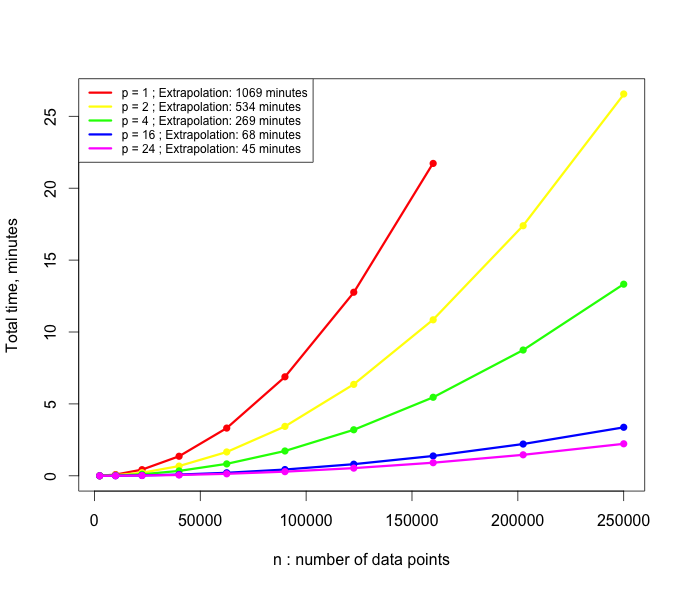
\includegraphics[width=0.5\textwidth]{./fig/comm_c1_timings.png} % requires the graphicx package
   \caption{example caption}
   \label{fig:comm_c1_timings}
\end{figure}

We executed 10 test cases for our communication-optimal and computational-optimal implementations for various numbers of processors. Figure~\ref{fig:comm_c1_timings} shows the timing results for our communication optimal implementation with the replication factor $c=1$. It depicts the distinctive $O(n^2)$ curve for the smaller number of processors $p$ (the horizontal axis is too small to show the shape of the curve for the larger $p$) and the expected reduction in time with increasing $p$. For each of these curves, we fit a line between total time and $n^2$ and then extrapolated the time required to run the large dataset of Figure~\ref{fig:herten} with $n=8.69\times10^6$. On the legend, the extrapolated time is written for each $p$ tested.  

Figure~\ref{fig:comm_allc_timings} compares $c=$ 1, 2, and 4. The effect of $c$ is not evident when looking at the total time. When breaking the total time down into time for reading the file, broadcasting the point data, shifting the point data, computing the squared differences, and reducing the bins (see Figure~\ref{fig:allc_breakdown}), it its evident that most of the total time is consumed by the computation stage. The effect of $c$ is more evident if only communication time is plotted (see Figure~\ref{fig:comm_allc_comm})

\begin{figure}[!ht]
   \centering
   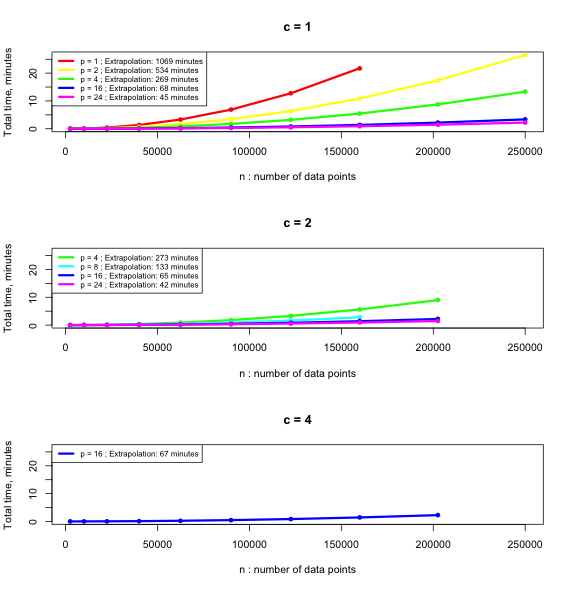
\includegraphics[width=0.5\textwidth]{./fig/comm_allc_timings.png} % requires the graphicx package
   \caption{example caption}
   \label{fig:comm_allc_timings}
\end{figure}

\begin{figure}[!ht]
   \centering
   \includegraphics[width=0.5\textwidth]{./fig/allc_breakdown.png} % requires the graphicx package
   \caption{example caption}
   \label{fig:allc_breakdown}
\end{figure}

\begin{figure}[!ht]
   \centering
   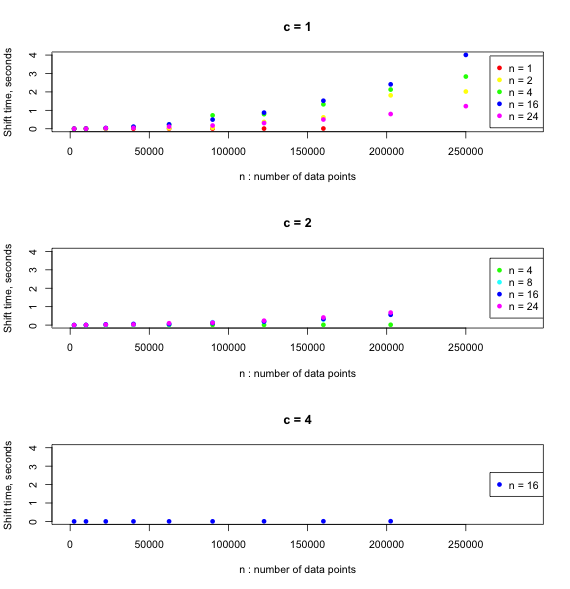
\includegraphics[width=0.5\textwidth]{./fig/comm_allc_comm.png} % requires the graphicx package
   \caption{example caption}
   \label{fig:comm_allc_comm}
\end{figure}

Due to computation consuming most of the total time, we next tried the computation optimal implementation. Figure~\ref{fig:comp_timings} shows the timing results for total time of our 10 test cases and for a range of processors. Again, the $O(n^2)$ curve is evident and we extrapolated the time required for our large data set. The total time for the computation optimal implementation is about half of that of the communication optimal implementation. Breaking down the total time for this computation optimal implementation (Figure~\ref{fig:comp_breakdown}), we can see that [...???...]. 

\begin{figure}[!ht]
   \centering
   \includegraphics[width=0.5\textwidth]{./fig/timing2.png} % requires the graphicx package
   \caption{example caption}
   \label{fig:comp_timings}
\end{figure}

Next, we looked at the scaling success (Figure~\ref{fig:scaling}). We divided the time $p=1$ by each larger $p$ and compared it to the $y=x$ line representing perfect scaling. It can be seen that for the larger test cases, there is near-perfect scaling. Although this is not the case for the smaller test cases, this is not really an issue because our program is designed for large data sets and small ones can be run in serial in reasonable time. 

Now that we are content with the performance of the computation optimal implementation, we increased $p$ and re-ran our test cases to determine the appropriate $p$ to run our large data set in a matter of seconds (instead of a day which is the quickest we could get with one node in our preliminary tests). Figure~\ref{}
